\documentclass[xcolor=x11names,compress,professionalfonts]{beamer}

%% General packages %%%%%%%%%%%%%%%%%%%%%%%%%%%%%%%%%%
\usepackage[utf8]{inputenc}
\usepackage{graphicx}
\usepackage{tikz}
\tikzset{% change default arrow tips
    >=latex
}
\usepackage{ifthen}

\usepackage{amsmath}
\usepackage{nicefrac}

\usepackage{color}

% compile child documents using this preamble
\usepackage{subfiles}

% compile child files with separate preambles, and include them in the document
\usepackage{standalone}

%%%%%%%%%%%%%%%%%%%%%%%%%%%%%%%%%%%%%%%%%%%%%%%%%%%%%%

\makeatletter
\setbeamertemplate{footline}
{
    \leavevmode%
    \hbox{%
        \begin{beamercolorbox}[wd=.333333\paperwidth,ht=2.25ex,dp=1ex,center]{author in head/foot}%
            \usebeamerfont{author in head/foot}\insertshortauthor
        \end{beamercolorbox}%
                \begin{beamercolorbox}[wd=.333333\paperwidth,ht=2.25ex,dp=1ex,center]{title in head/foot}%
            \usebeamerfont{title in head/foot}\insertshorttitle
        \end{beamercolorbox}%
        \begin{beamercolorbox}[wd=.333333\paperwidth,ht=2.25ex,dp=1ex,right]{date in head/foot}%
            \usebeamerfont{date in head/foot}\insertshortdate{}\hspace*{2em}
            \insertframenumber{} / \inserttotalframenumber\hspace*{2ex} 
        \end{beamercolorbox}}%
        \vskip0pt%
    }
    \makeatother


%% Beamer Layout %%%%%%%%%%%%%%%%%%%%%%%%%%%%%%%%%%
\useoutertheme[subsection=false,shadow]{miniframes}
\useinnertheme{rectangles}

\setbeamertemplate{navigation symbols}{}%remove navigation symbols

\author{Nicolas Macé}

\newcommand{\btVFill}{\vskip0pt plus 1filll}%place an element at the bottom of the page

\usepackage{libertine}
\usepackage[T1]{fontenc}

\setbeamerfont{title like}{shape=\scshape}
\setbeamerfont{frametitle}{shape=\scshape}

\setbeamercolor*{lower separation line head}{bg=DeepSkyBlue4} 
\setbeamercolor*{normal text}{fg=black,bg=white} 
\setbeamercolor*{alerted text}{fg=red} 
\setbeamercolor*{example text}{fg=black} 
\setbeamercolor*{structure}{fg=black} 
 
\setbeamercolor*{palette tertiary}{fg=black,bg=black!10} 
\setbeamercolor*{palette quaternary}{fg=black,bg=black!10} 

\renewcommand{\(}{\begin{columns}}
\renewcommand{\)}{\end{columns}}
\newcommand{\<}[1]{\begin{column}{#1}}
\renewcommand{\>}{\end{column}}

\definecolor{BostonBlue}{HTML}{00688B}
\definecolor{Complementary}{HTML}{8B2300}

% letters A and B appearing in the qp chains
\newcommand{\A}{\textcolor{BostonBlue}{A}}
\newcommand{\B}{\textcolor{Complementary}{B}}

\renewcommand{\ss}[1]{\scriptsize{\text{#1}}}
%%%%%%%%%%%%%%%%%%%%%%%%%%%%%%%%%%%%%%%%%%%%%%%%%%

\usepackage{braket}
% compile child documents using this preamble
\usepackage{subfiles}

%%%My Math

\newcommand{\pd}[2]{\frac{\displaystyle \partial #1}{\displaystyle\partial #2}} % for partial derivatives
\renewcommand{\d}[1]{\mathrm{d}#1}

\begin{document}

\begin{frame}
\title{{\fontsize{14}{60}\selectfont Exact results on electronic wavefunctions of 2D quasicrystals}}

\author{Nicolas Macé, Anuradha Jagannathan, Frédéric Piéchon}

\institute % (optional)
{
  Laboratoire de Physique des Solides\\
  Université Paris-Saclay
}

\date{September 20, 2016}

\titlepage

\btVFill
\begin{columns}
\begin{column}{2cm}
~\\
~\\
~\\
~\\
\raggedright

\includegraphics[scale=.15]{img/LogoUPSUD.png}
\end{column}
\begin{column}{6cm}
\centering
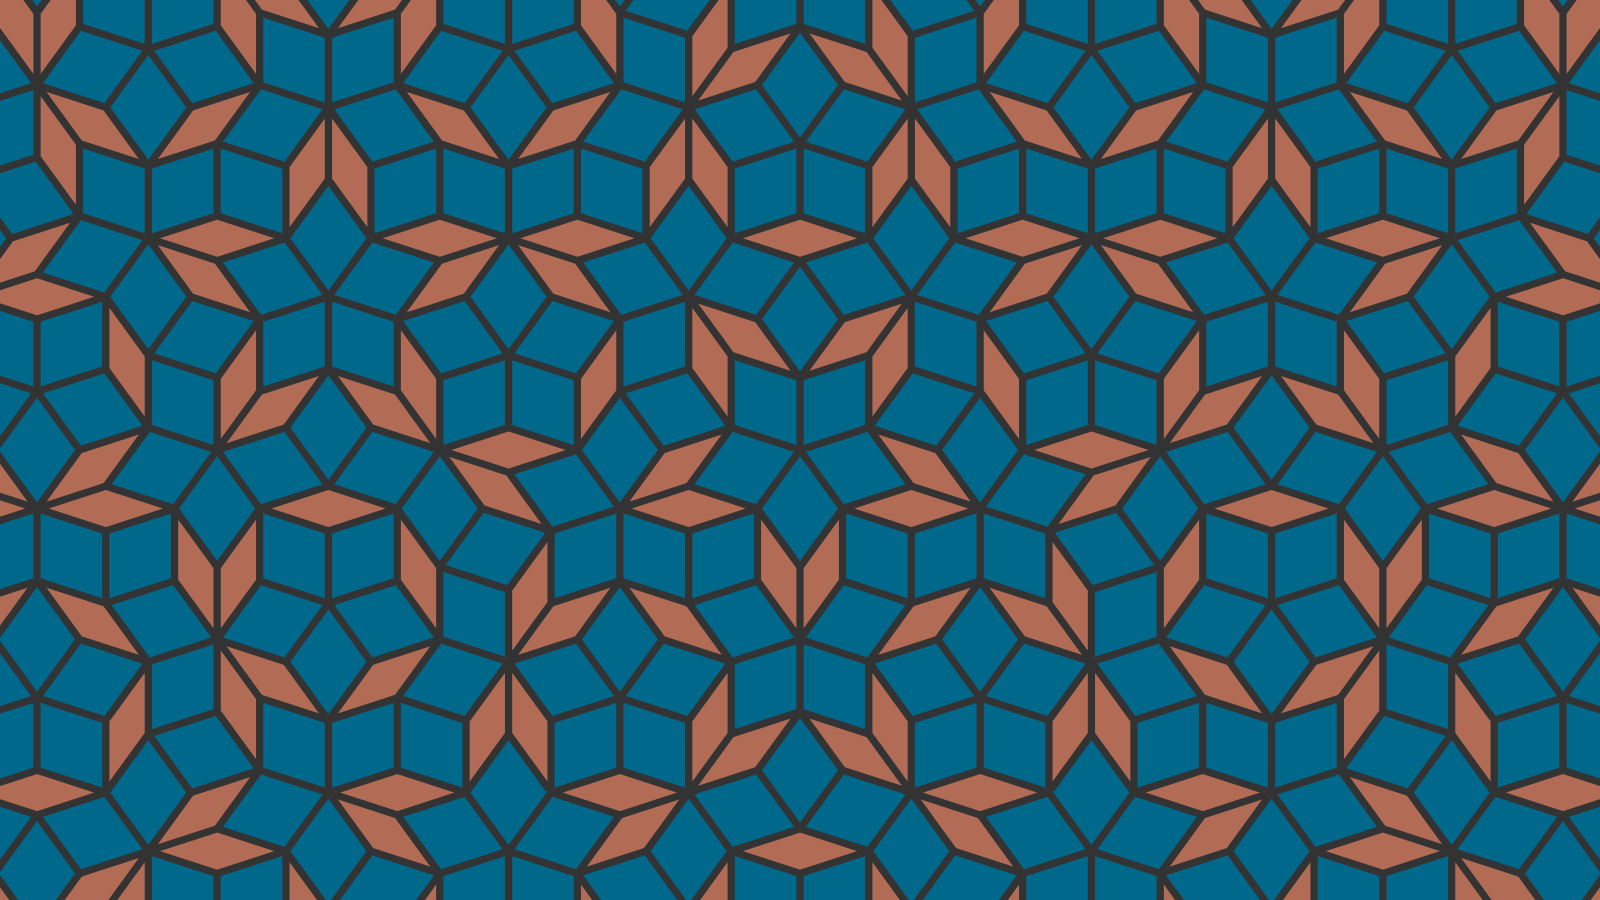
\includegraphics[width=.7\textwidth]{img/cover.png}
\end{column}
\begin{column}{2cm}
~\\
~\\
~\\
~\\
\raggedleft

\includegraphics[scale=.15]{img/logo-lps.jpg}
\end{column}
\end{columns}
\end{frame}

\begin{frame}{Electrons on quasicrystals}
\begin{itemize}
	\item In 1D (quasiperiodic chains): electronic spectrum and wavefunctions are well known. 
	\item In 2D and 3D: many numerical investigations, but almost no exact results.
\end{itemize}
$\rightarrow$ recent (big!) improvement: Kalugin, Katz (2014) guessed the groundstate of a large class of 2D models.

\begin{itemize}
	\item What does this groundstate look like?
	\item Which new insights does it bring us?
\end{itemize} 
\end{frame}

\begin{frame}
\frametitle{Toy models of quasicrystals}
We want to model:
\begin{itemize}
	\item a single electron (ie we do not consider interactions)
	\item on a quasiperiodic tiling, in 1D or in 2D
	\item in the simplest possible way : tight-binding model with nearest neighbors hoppings only
\end{itemize}

\begin{columns}
\<{4cm}
\[
	i \frac{\partial \phi_m}{\partial t}(t) = \sum_{n \in V(m)} t_{m,n} \phi_n(t)
\]
$|\phi_m(t)|^2= $ proba to be on atom $m$ at time $t$.
\>

\<{2cm}
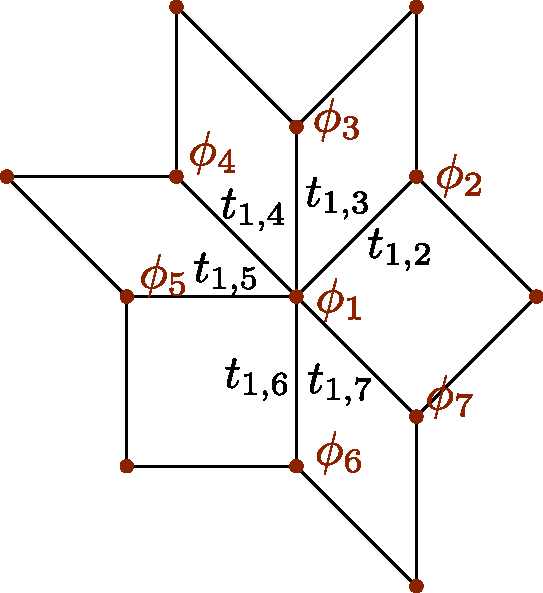
\includegraphics[scale=0.34]{img/ham_example.pdf}
\>

\<{3cm}
Solve for the stationary states (or eigenstates):
\[
	E \psi_m = \sum_{n \in V(m)} t_{m,n} \psi_n
\]
\>
\end{columns}

Challenge: find a proper description of these eigenstates... 
\end{frame}

\begin{frame}
\frametitle{Outline}
\tableofcontents[hideallsubsections]
\end{frame}

\begin{frame}
\frametitle{Periodic and disordered models}
\begin{itemize}
	\item Eigenstates on periodic materials: 
	\begin{itemize}
		\item Plane waves 
		\item \textbf{uniform} probability $\rightarrow$ \textbf{extended states}
	\end{itemize}
	\subfile{img/periodic_chain.tex}
	\item Eigenstates on disordered materials: 
	\begin{itemize}
		\item Evanescent waves
		\item  \textbf{exponentially decreasing} probability $\rightarrow$ \textbf{localized states}
	\end{itemize}
	\subfile{img/disordered_chain.tex}
\end{itemize}
\textbf{What about quasiperiodic materials?}

\textcolor{Complementary}{We will see on examples their electrons are somewhat \textbf{in between}: the wavefunctions have local power law decay, they are \textbf{critical}}
\end{frame}

\section{1D models: a ``baby example''}
%Each section needs a subsection for the small points on top to show up
\subsection{Dummy}

\begin{frame}{The Fibonacci chain}
		The geometrical model: a chain of two letters generated by the substitution
	\[	
	M: \left\{\begin{array}{ll} \A \to & \A \B \\ \B \to & \A
	\end{array}\right.	
	\]
		
{\centering
$M^{\infty}(\A) = \dots\A\B\A\B\A\A\B\A\A\B\A\B\A\A\B\A\B\A\dots $

}
		
		The corresponding chain of atoms:
		
		{\centering
		\subfile{img/fibo_chain.tex}
		
		}
The Schrödinger equation for the eigenstate of energy $E$:
\[
	 t_{m-1,m} \psi_{m-1} + t_{m,m+1}\psi_{m+1} = E \psi_{m}
\]
\[
	t_{m-1,m} = t_s \text{~or~} t_w \text{~we introduce the ratio $\rho = t_w / t_s$}
\]
What can be say about the spectrum/eigenstates of this model?
\end{frame}

\begin{frame}{Spectrum and eigenstates}
\begin{itemize}
	\item The spectrum is scale invariant (or multifractal)
	
{\centering
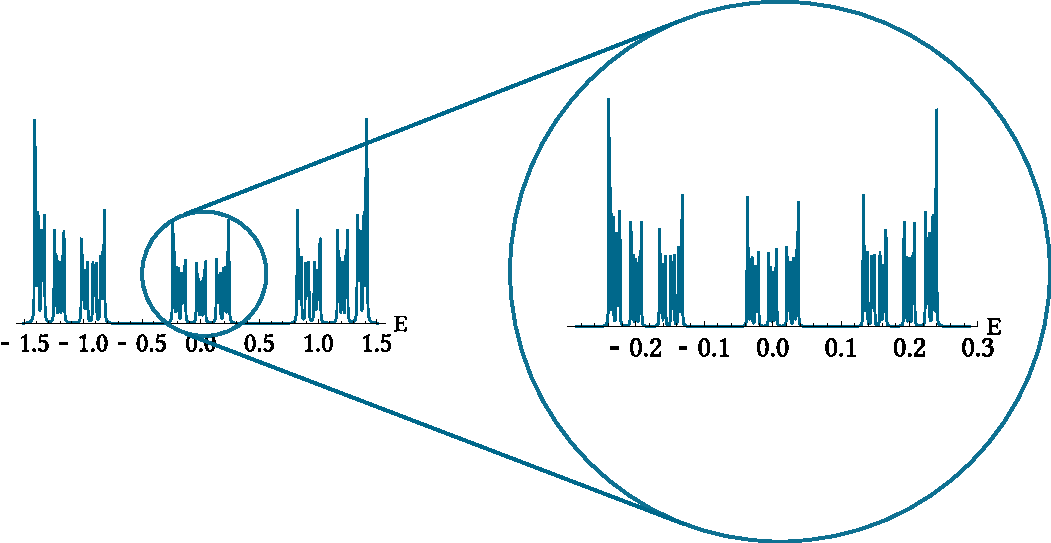
\includegraphics[scale=.5]{img/ldos.pdf}

}
	\item The eigenstates are all critical (neither localized nor extended)
\end{itemize}
What is the structure of these critical states?
\end{frame}

\begin{frame}{A baby example: the eigenstate at zero energy}
\begin{itemize}
	\item Schrödinger equation for the $E=0$ state:
	\[
	t_{m-1,m} \psi_{m-1} + t_{m,m+1}\psi_{m+1} = 0
	\]
	\item If we know the wavefunction on one site we know it on the next
	\begin{columns}
	\<{6cm}
	\[
	\psi_{m+1} = -\frac{t_{m-1,m}}{t_{m,m+1}} \psi_{m-1}
	\]
	\>
	\<{5cm}
	\subfile{img/hop_E0.tex}
	\>
	\end{columns}
	\only<1>{
	\item There are 4 possible cases:
	
	\centering
	 \subfile{img/hop_1.tex}
	 }
	\only<2>{
	\item Introduce $A_{m-1,m+1}$, the \textbf{arrow} from $m-1$ to $m+1$:
	\begin{columns}
	\<{5cm}
	\centering
	 \subfile{img/hop_2.tex}
	 \>
	 \<{5cm}
	Then, $\boxed{\psi_{m+1} = \rho^{A_{m-1,m+1}} \psi_{m-1}}$
	 \>
	 \end{columns}
	 }
\end{itemize}
\end{frame}

\begin{frame}{The field of arrows and the field of heights}
Iterating $\psi_{m+1} = \rho^{A_{m-1,m+1}} \psi_{m-1}$,
\[
	\psi_{m} = \psi_0 \rho^{h(m)}
\]
Where $h$ is \textbf{the field of heights}, the integral of the field of arrows:
\[
	h(m) = \sum_{n=1}^{m/2} A_{2n-2, 2n}
\]

Example (piece of the Fibonacci chain):
\subfile{img/field_of_heights.tex}


\end{frame}

\begin{frame}{Back to the special cases, with arrows!}
\begin{itemize}
	\item Periodic chain: 
	\subfile{img/periodic_chain_arrows.tex}
	\begin{itemize}
		\item Arrows $= 0 \implies h(m) = 0 \implies \psi_m = \psi_0 \rho^{0} = $ cst  
		\item \textbf{uniform} probability $\rightarrow$ \textbf{extended states}
	\end{itemize}
	\item Disordered chain: 
	\subfile{img/disordered_chain_arrows.tex}
	\begin{itemize}
		\item Arrows randomly distributed $\implies h(m) \sim \langle A \rangle \times m \implies \psi_m \sim \rho^{\langle A \rangle \times m} \sim e^{- m/\xi}$ with $\xi^{-1} = |\log \rho| \langle A \rangle$
		\item  \textbf{exponentially decreasing} amplitude $\rightarrow$ \textbf{localized states}
	\end{itemize}
\end{itemize}
$\rightarrow$ expected behavior in both cases.

What happens for a quasiperiodic chain?
\end{frame}

\begin{frame}{The $E=0$ state is not localized}
\begin{columns}
\<{6cm}
Apply the substitution three times:
	\[	
	M^3: \left\{\begin{array}{ll} \A \to & \A \B \A \B \A \\ \B \to & \A \B \A
	\end{array}\right.	
	\]
\>
\<{6cm}
{
\centering
\subfile{img/atomic_inflation_no_localization.tex}
}
\>
\end{columns}
$\rightarrow$ the height is invariant under the substitution $M^3$: it doesn't change on the preexisting sites
\begin{itemize}
	\item the wavefunction doesn't change on the preexisting sites
	\item these preexisting sites get arbitrary far apart as we iterate the substitution 
\end{itemize}
$\rightarrow$ we can find the electron with high probability arbitrarily far from the origin: \textbf{the wavefunction cannot be localized.}
\end{frame}

\begin{frame}{The $E=0$ state is not extended}
{

\centering
\subfile{img/atomic_inflation_no_extension.tex}
}

\begin{columns}
\<{6cm}
{\centering
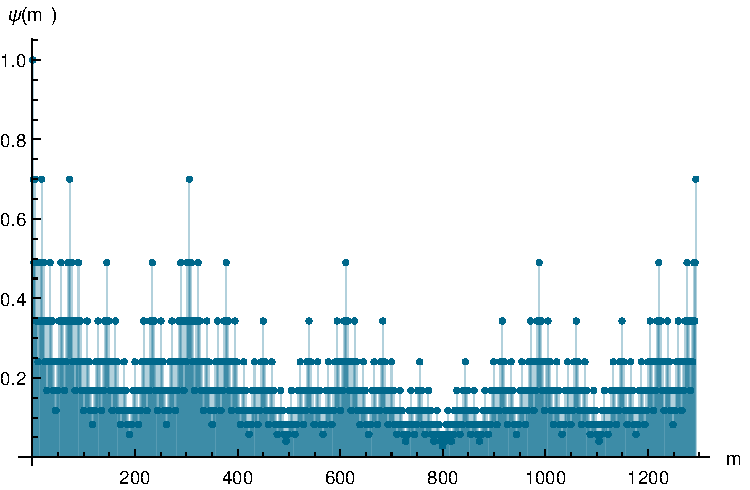
\includegraphics[scale=.5]{img/wavefunction.pdf}

}
\>

\<{6cm}
Local scale invariance:
\[
	\psi_{a \times m} = b \times \psi_{m} 
\]
$\rightarrow$ local \textbf{power law decay}
\[
\psi_{r_n} \sim r_n^\alpha, ~(\alpha = \log b/\log a)
\]
$\rightarrow$ \textbf{wavefunction cannot be extended}
\>
\end{columns}

\end{frame}

\begin{frame}{Cut and project chains: a summary}
\begin{itemize}
	\item The $E=0$ wavefunction of cut and project chains can be described by a \textbf{height field}
	\item The height field is the integral of an \textbf{arrow field}, which is quasiperiodic
	\item As a result, \textbf{the wavefunction is critical}: it behaves locally as a power law
	\item On a patch of the tiling of size $L$, maximal height scales as $\log L$, typical height as $\sqrt{\log L}$
\end{itemize}
We will find again all these features in 2D!
\end{frame}

\section{2D models: the ``grown-up example''}
\subsection{Dummy}

\begin{frame}{2D tilings}
We consider the Penrose and the Ammann-Beenker tilings.
\begin{columns}
\begin{column}{5cm}
{\centering
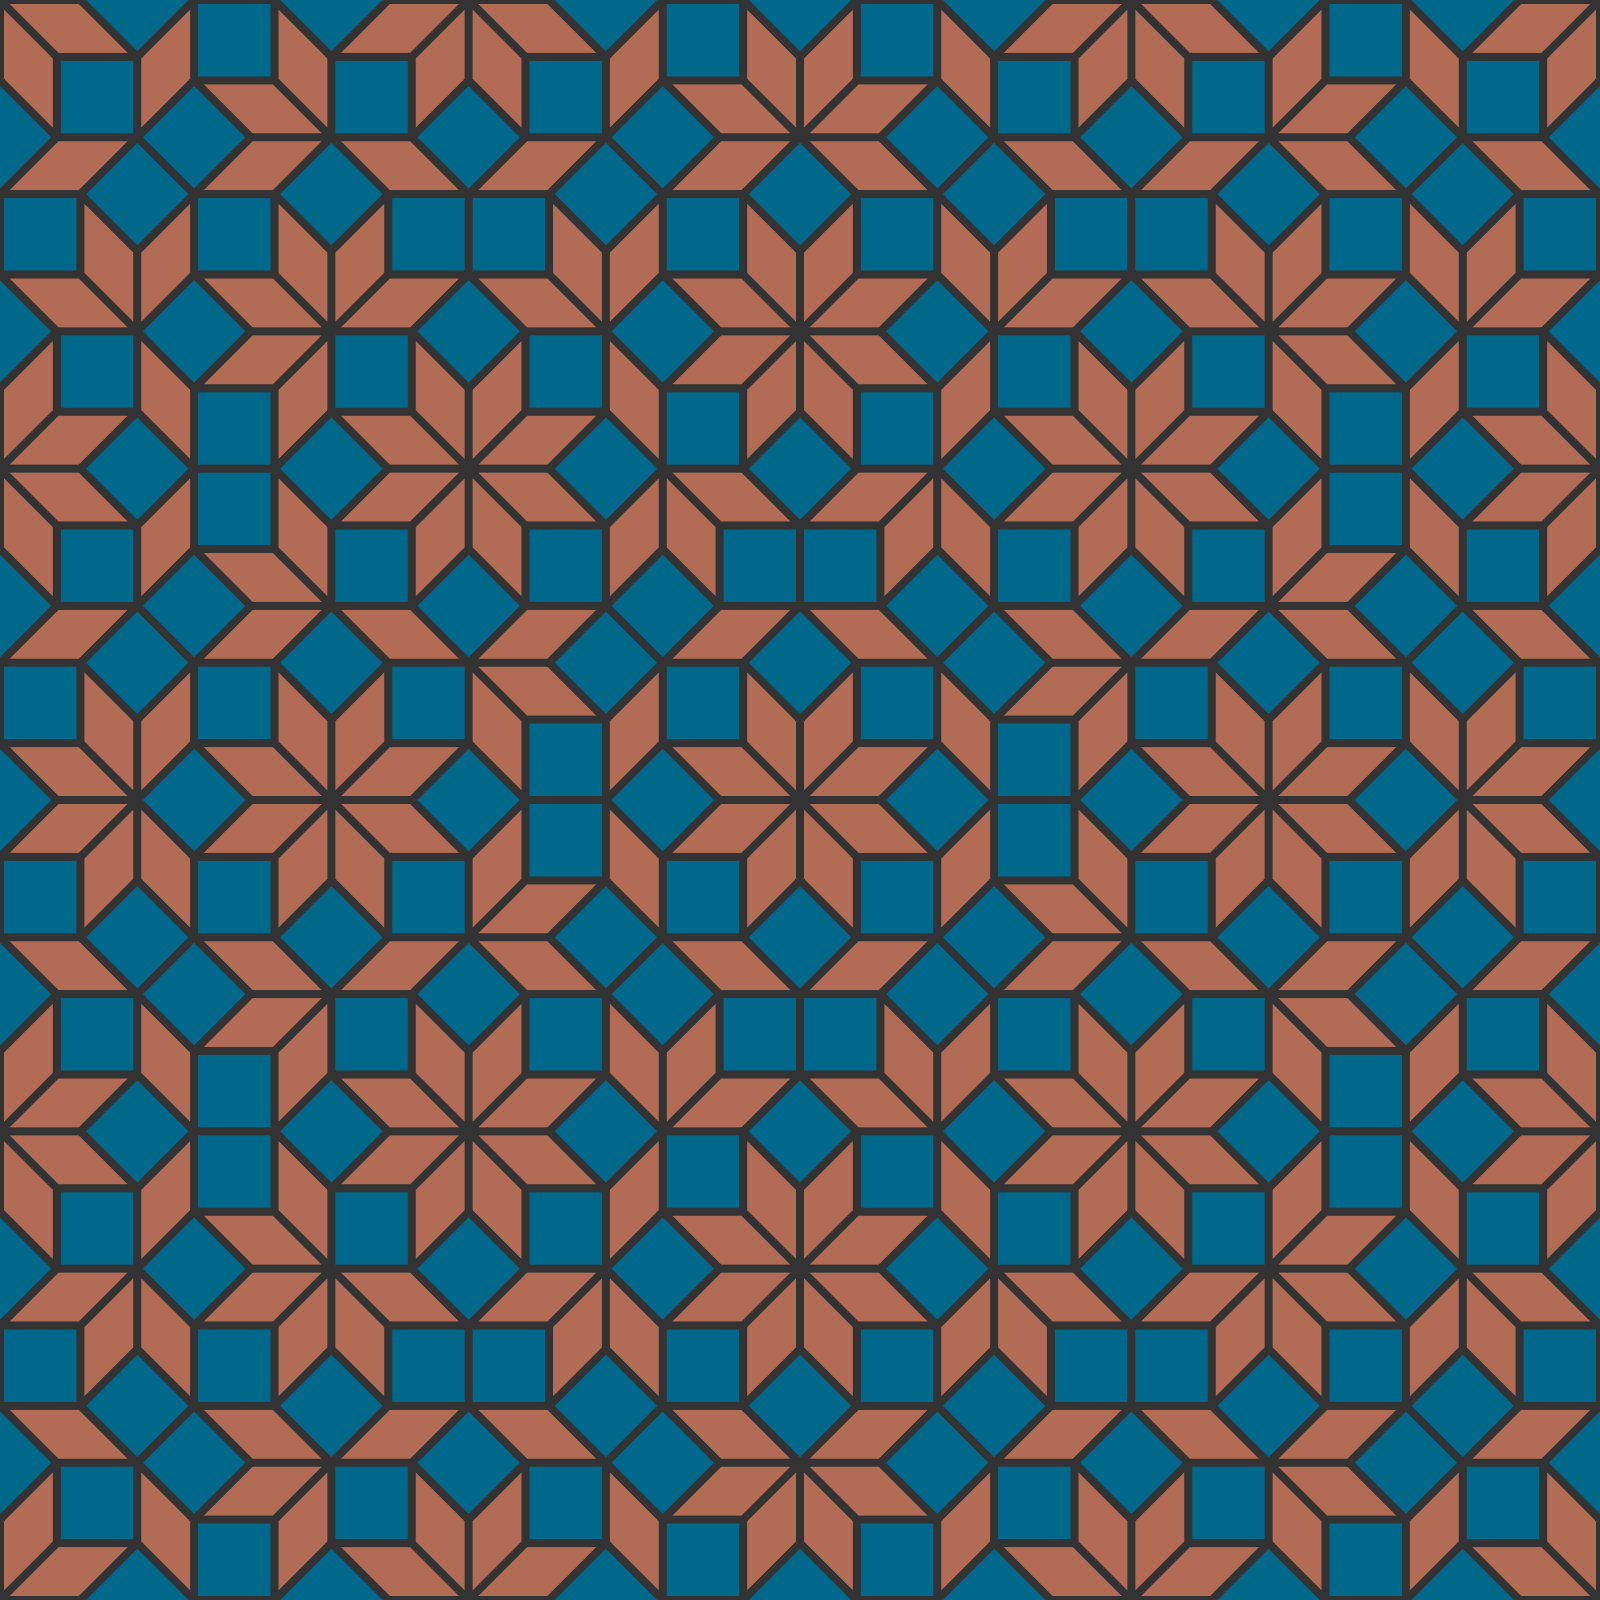
\includegraphics[scale=.08]{img/ammann-beenker.png}

}
\end{column}
\begin{column}{5cm}
{\centering
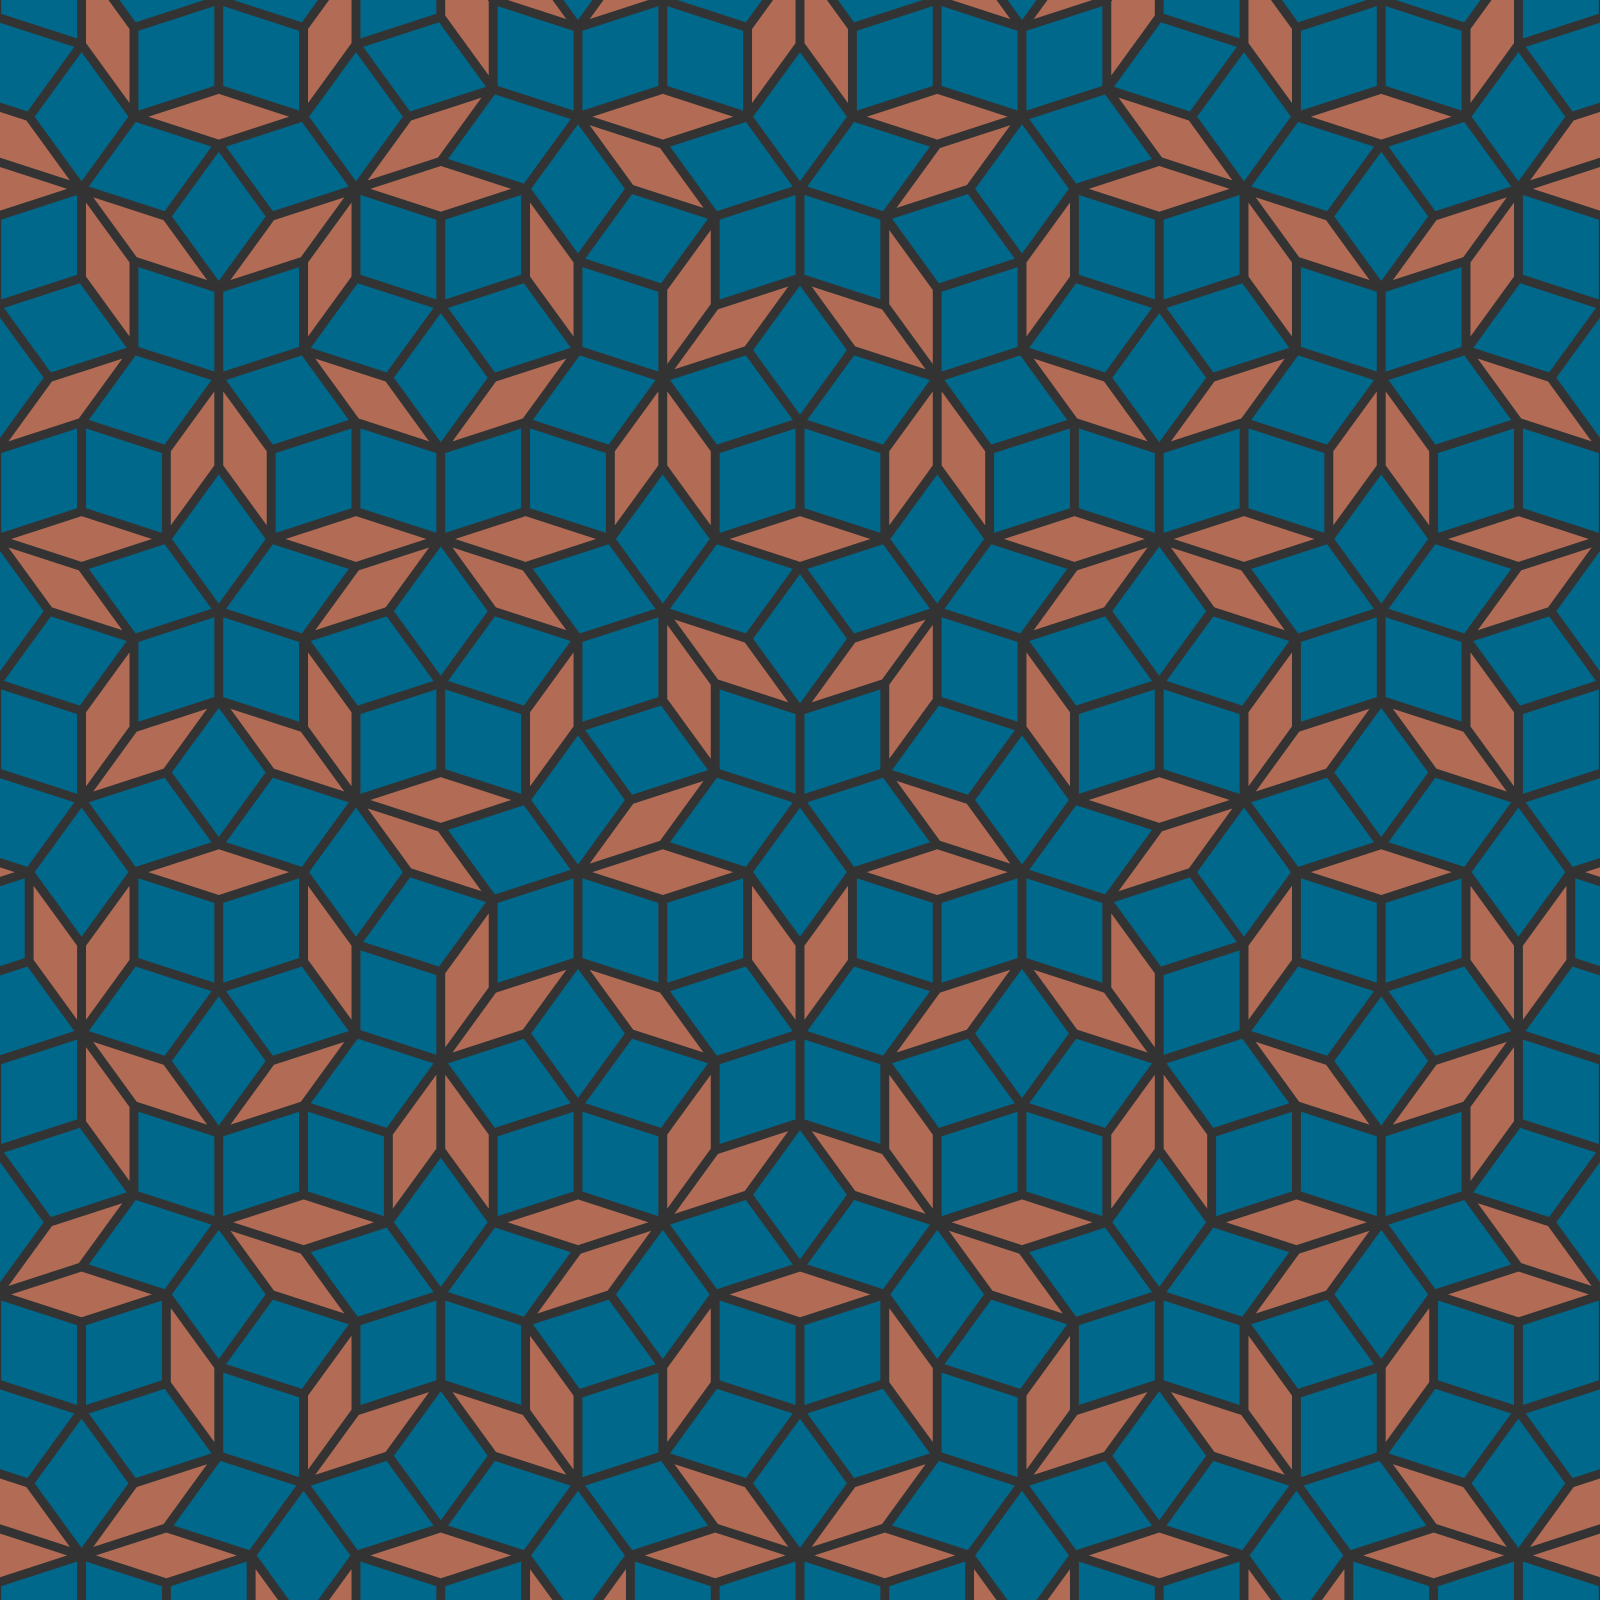
\includegraphics[scale=.08]{img/penrose.png}

}
\end{column}
\end{columns}
Model:
\[
	E \psi_m = V_m \psi_m + t\sum_{n \in V(m)} \psi_n
\]
The quasiperiodic features are encoded in the adjacency of the vertices.
\end{frame}

\begin{frame}{What is known}

{\centering
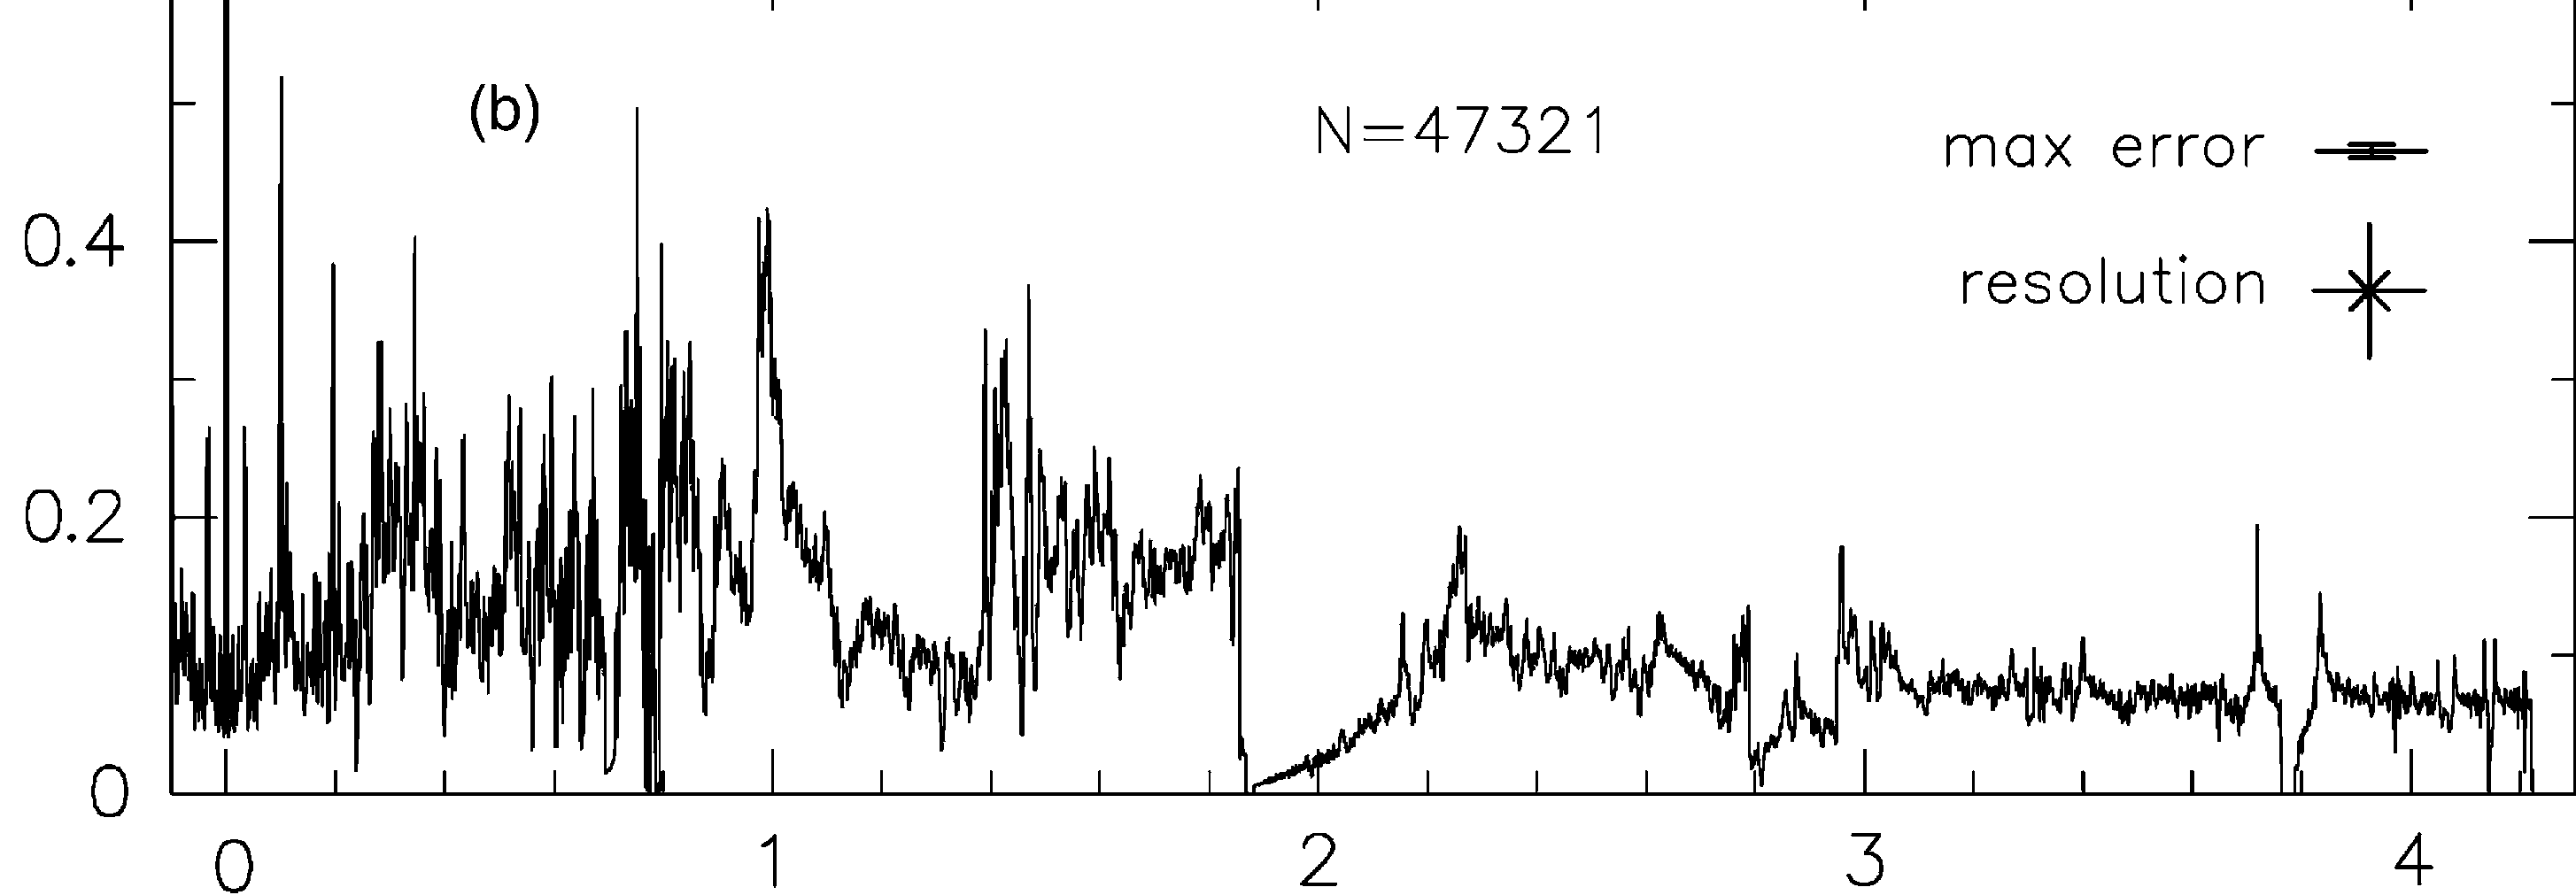
\includegraphics[scale=.1]{img/idos_AB_small.png}

}
\begin{itemize}
	\item Spectrum is more regular: only a few gaps, no apparent fractal structure
	\item $E = 0$ eigenstates are localized: cannot hope to describe them with arrows.
	\item The other states are critical (numerical result)
\end{itemize}
$\rightarrow$ can we introduce a field of arrows to describe some of these critical wavefunctions?
\end{frame}

\begin{frame}{A natural field of arrows}

\end{frame}

\begin{frame}{Inflation and the field of arrows}
Here we focus on the AB example, but everything works the same for Penrose.
\begin{itemize}
	\item Arrows $\leftrightarrow$ matching rules for the tiles 
	\item Matching rules are enforced by the inflation rules $\rightarrow$ we should be able to study the properties of the arrows via the inflation (just like in 1D)
	\item From the inflation rules, we deduce the maximal height $\sim \log L$
	\item Statistics of the heights $P_\mu^{l}(h)$ obeys a diffusion-like equation where $l$ plays the role of time and $h$ the role of space
	\item $\rightarrow$ typical height is $\sim \sqrt{\log L}$
\end{itemize}
So we understand everything about Stutherland's wavefunction, but the model has been built for this wavefunction to exist. 
Can we use this field of arrows to describe wavefunctions on more realistic models?
Yes: Pavel.
\end{frame}

\begin{frame}{Characterization of the groundstate wavefunction}
\begin{itemize}
	\item We go back to the model with no local potentials. 
	\item From the plot of the groundstate: we see a complicated local structure (role of the local environment) and the phason line (role of the arrow field)
	\item Indeed, the wf decomposes into a local part and an arrow part (this was guessed from involved algebraic arguments).
	\item Computation of the IPR scaling and the multifractal exponents: the local part doesn't play any role $\rightarrow$ exponents only sensitive to the arrow part, ie to the quasiperiodicity!
	\item Remains valid for a larger class of models $H = \sum_{\langle i, j \rangle} \ket{i} \bra{j} + V_i \ket{i} \bra{i} $
\end{itemize}
\end{frame}

\begin{frame}{Conclusion}
\begin{itemize}
	\item Non-interacting eigenstates on quasicrystals are generically critical: here we were able to understand it for some specific states, both in 1D and 2D.
	\item On our examples, wavefunction construction involves a geometrical quasiperiodic function, the field of arrows.
	\item Its integral, the height function, has logarithmic growth,
	\item As a result, the wavefunction is critical: it has a local power law behavior.
\end{itemize}
Perspectives:
\begin{itemize}
	\item What happens for the grounstate of other quasicrystals, like the dodecagonal ones?
	\item For Penrose and AB, the arrow field cannot be used to describe other states. What extra ingredients are required?
\end{itemize}
\end{frame}

\begin{frame}{More perpsectives!}
\begin{itemize}
	\item A plot of the state just below the gap, with its quasiperiodic array of lines of zeros, that remain to be understood!
\end{itemize}
\end{frame}

%%%%%%%%%%%% Extra slides %%%%%%%%%%%%%
\begin{frame}{Cut and project chains are special!}
Consider the chain constructed by the substitution
\begin{align*}
	A & \to ABBB \\
	B & \to A
\end{align*}
\begin{columns}
\<{6cm}
\begin{itemize}
	\item This substitution cannot be built by cut and project (because it is non-Pisot).
	\item Height resembles a random walk, and typical height $\sim \sqrt{L}$
	\item As a result, the wavefunction is localized! 
\end{itemize}
\>
\<{6cm}
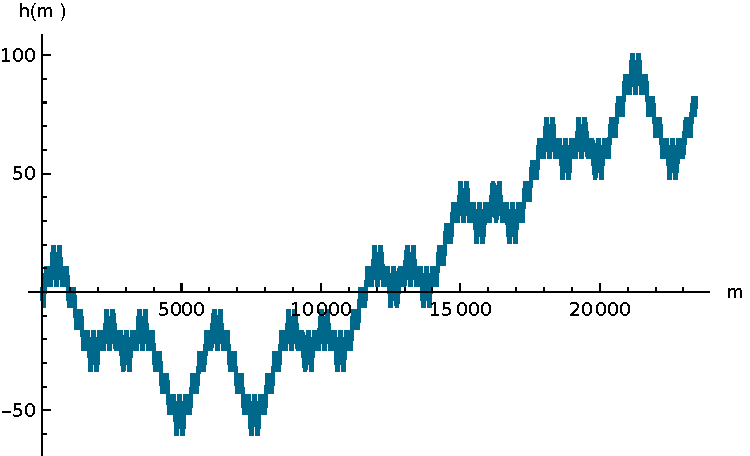
\includegraphics[scale=.5]{img/heightsB3.pdf}
\>
\end{columns}
$\rightarrow$ criticality is sensitive to the \textbf{complexity} of the tiling
\end{frame}



\end{document}